\documentclass{beamer}

\usepackage{cmap}
\usepackage[T1,T2A]{fontenc}
\usepackage[utf8]{inputenc}
\usepackage[russian]{babel}

\mode<presentation> {
\usetheme{Madrid}
\setbeamertemplate{caption}[numbered]
}

\usepackage{graphicx} % Allows including images
\usepackage{booktabs} % Allows the use of \toprule, \midrule and \bottomrule in tables

\title[Системное программирование]{Утилита htop}

\author{Мартынов Семён}
\institute[СПб ПУ]
{
Санкт-Петербургский политехнический университет Петра Великого\\
\medskip
\textit{semen.martynov@gmail.com}
}
\date{\today}

\begin{document}

\begin{frame}
\titlepage
\end{frame}

\begin{frame}
\frametitle{Содержание}
\tableofcontents
\end{frame}

%------------------------------------------------
\section{Введение}
%------------------------------------------------

\begin{frame}
\frametitle{Введение}

Htop написан на языке Си и использует для отображения библиотеку Ncurses. Показывает динамический список системных процессов, список обычно выравнивается по использованию ЦПУ.

\begin{figure}
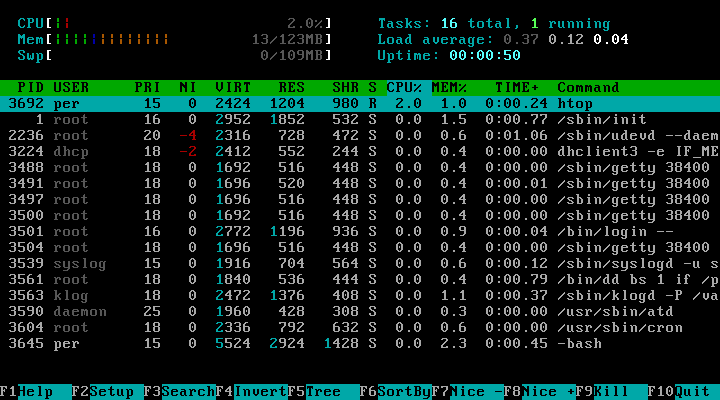
\includegraphics[scale=0.4]{res/Htop}
\caption{Системный монитор htop}
\end{figure}

\end{frame}

%------------------------------------------------
\section{Виртуальная файловая система procfs}
%------------------------------------------------

\begin{frame}
\frametitle{Виртуальная файловая система procfs}

Procfs позволяет получить доступ к информации о системных процессах из ядра.

Она создает двухуровневое представление пространств процессов:
\begin{itemize}
\item На верхнем уровне процессы представляют собой директории, именованные в соответствии с их pid.
\item На нижнем - файлы со значениями.
\end{itemize}

\begin{figure}
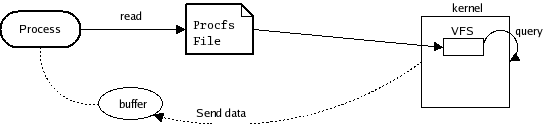
\includegraphics[scale=0.6]{res/ProcessFileSystem}
\caption{Файловая система procfs}
\end{figure}

\end{frame}

%------------------------------------------------
\section{Процессы}
%------------------------------------------------

\begin{frame}
\frametitle{Процессы}

\begin{figure}
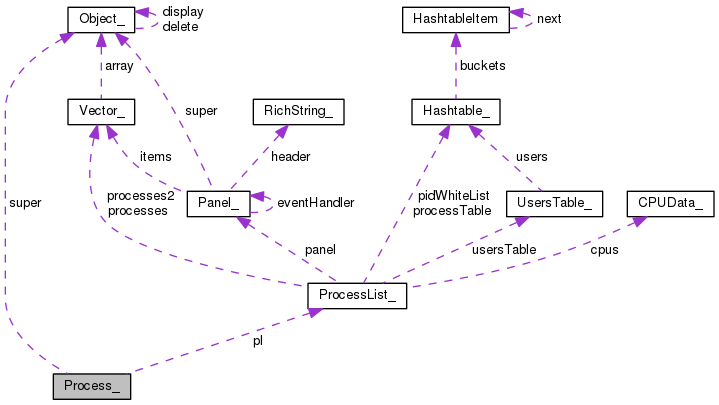
\includegraphics[scale=0.47]{res/process.png}
\caption{Граф взаимодействия для структуры Process}
\end{figure}

\end{frame}

%------------------------------------------------
\section{Измерение уровня заряда батарейки}
%------------------------------------------------

\begin{frame}
\frametitle{Измерение уровня заряда батарейки}

\begin{figure}
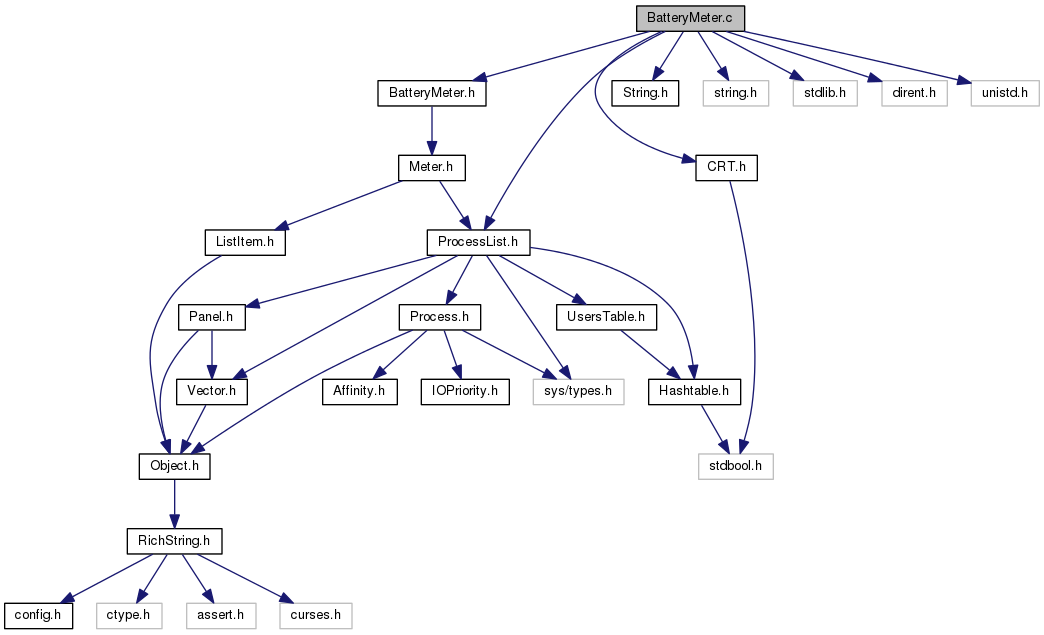
\includegraphics[scale=0.3]{res/battery_meter.png}
\caption{Граф включения для файла BatteryMeter.c}
\end{figure}

\end{frame}
%------------------------------------------------
\section{Мониторинг времени}
%------------------------------------------------

\begin{frame}
\frametitle{Мониторинг времени}

\begin{figure}
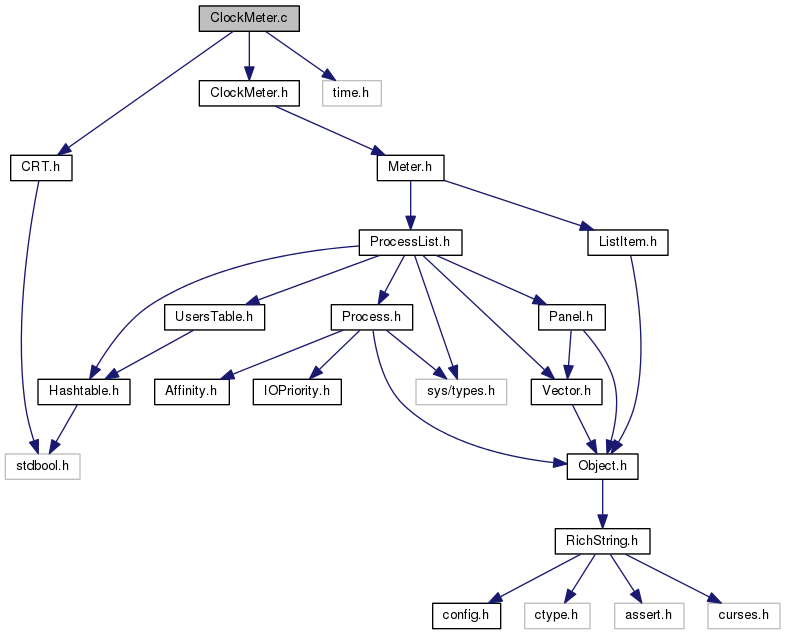
\includegraphics[scale=0.35]{res/clock_meter.png}
\caption{Граф включения для файла ClockMeter.c}
\end{figure}

\end{frame}
%------------------------------------------------
\section{Центральный процессор}
%------------------------------------------------

\begin{frame}
\frametitle{Центральный процессор}

\begin{figure}
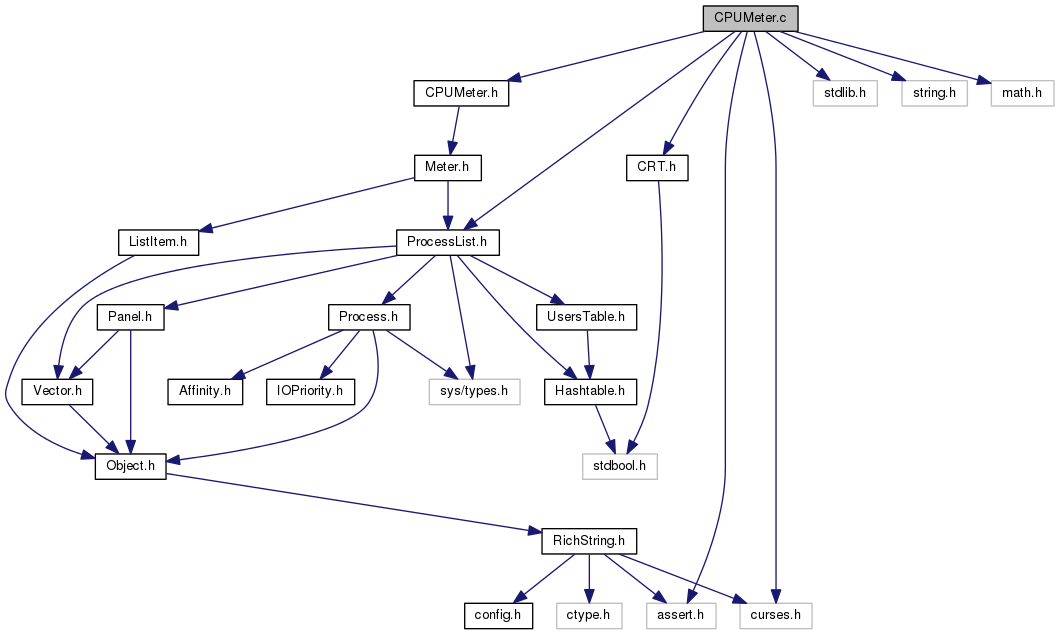
\includegraphics[scale=0.3]{res/cpu_meter.png}
\caption{Граф включения для файла ClockMeter.c}
\end{figure}

\end{frame}
%------------------------------------------------
\section{Имя устройства (хоста)}
%------------------------------------------------

\begin{frame}
\frametitle{Имя устройства (хоста)}

\begin{figure}
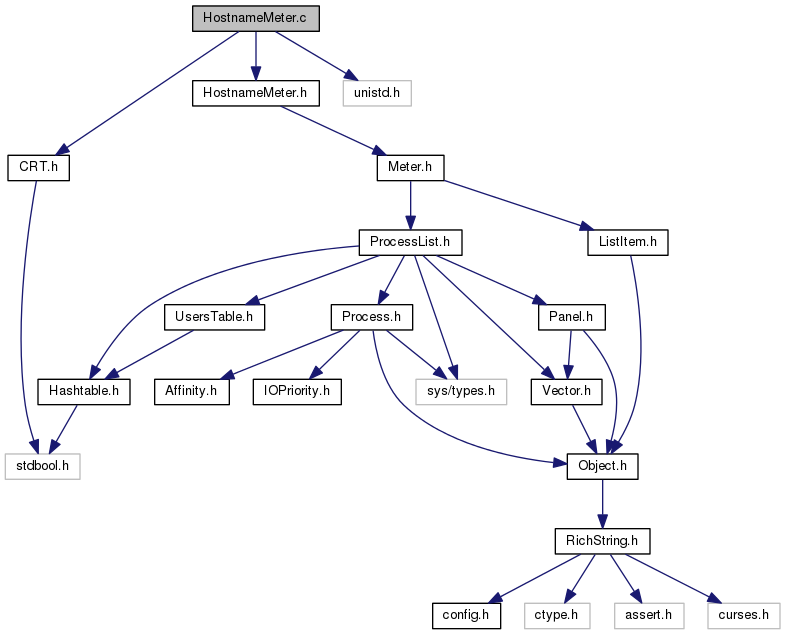
\includegraphics[scale=0.3]{res/hostname_meter.png}
\caption{Граф включения для файла HostnameMeter.c}
\end{figure}

\end{frame}
%------------------------------------------------
\section{Измерение средней загрузки}
%------------------------------------------------

\begin{frame}
\frametitle{Измерение средней загрузки}

\begin{figure}
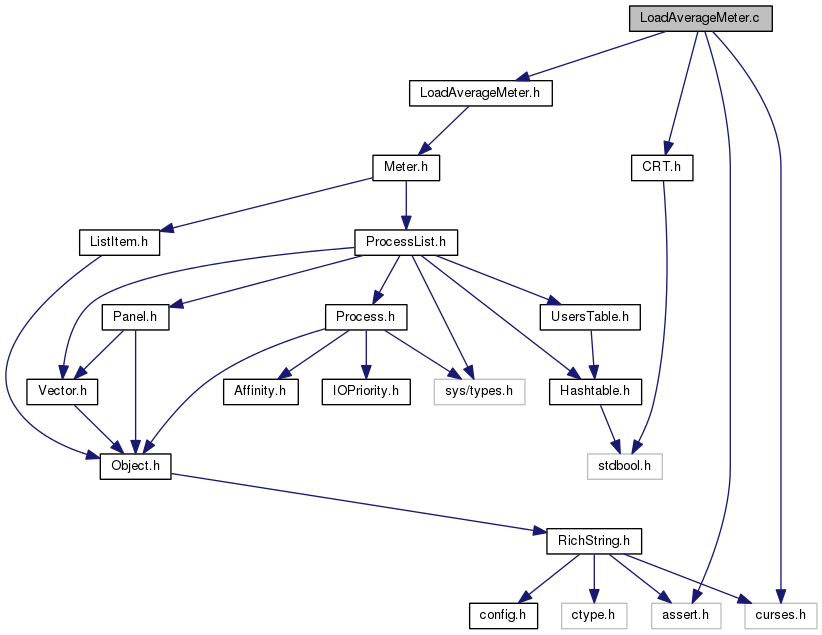
\includegraphics[scale=0.3]{res/load_average_meter.png}
\caption{Граф включения для файла LoadAverageMeter.c}
\end{figure}

\end{frame}
%------------------------------------------------
\section{Измерение уровня использования памяти}
%------------------------------------------------

\begin{frame}
\frametitle{Измерение уровня использования памяти}

\begin{figure}
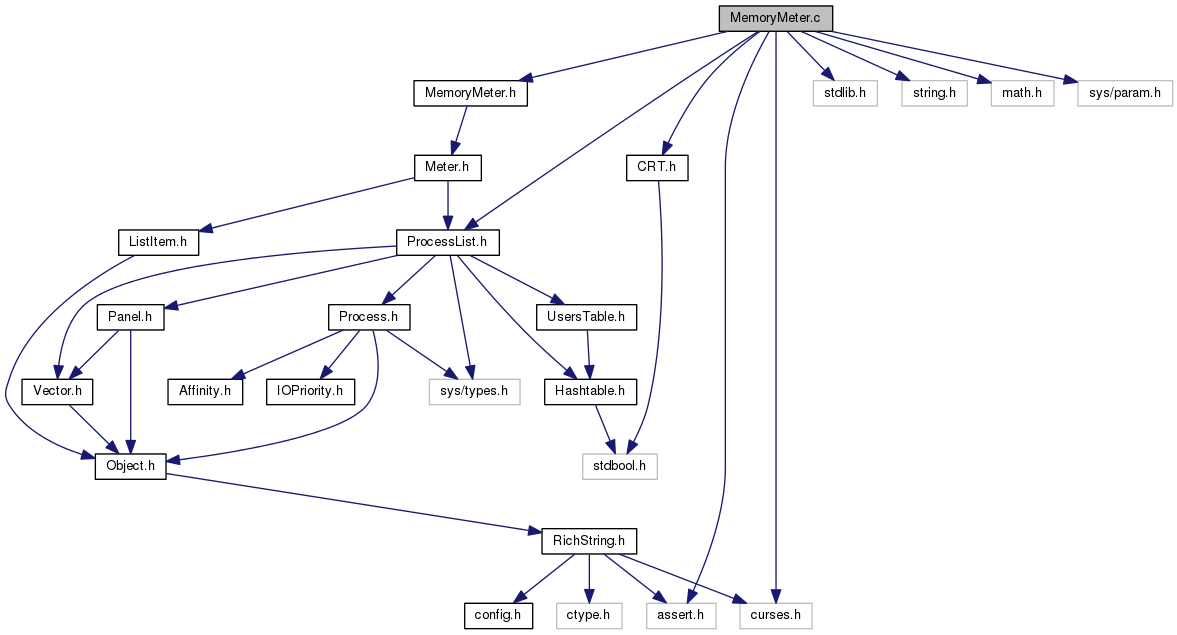
\includegraphics[scale=0.3]{res/memory_meter.png}
\caption{Граф включения для файла MemoryMeter.c}
\end{figure}

\end{frame}
%------------------------------------------------
\section{Измерение уровня использования области подкачки}
%------------------------------------------------

\begin{frame}
\frametitle{Измерение уровня использования области подкачки}

\begin{figure}
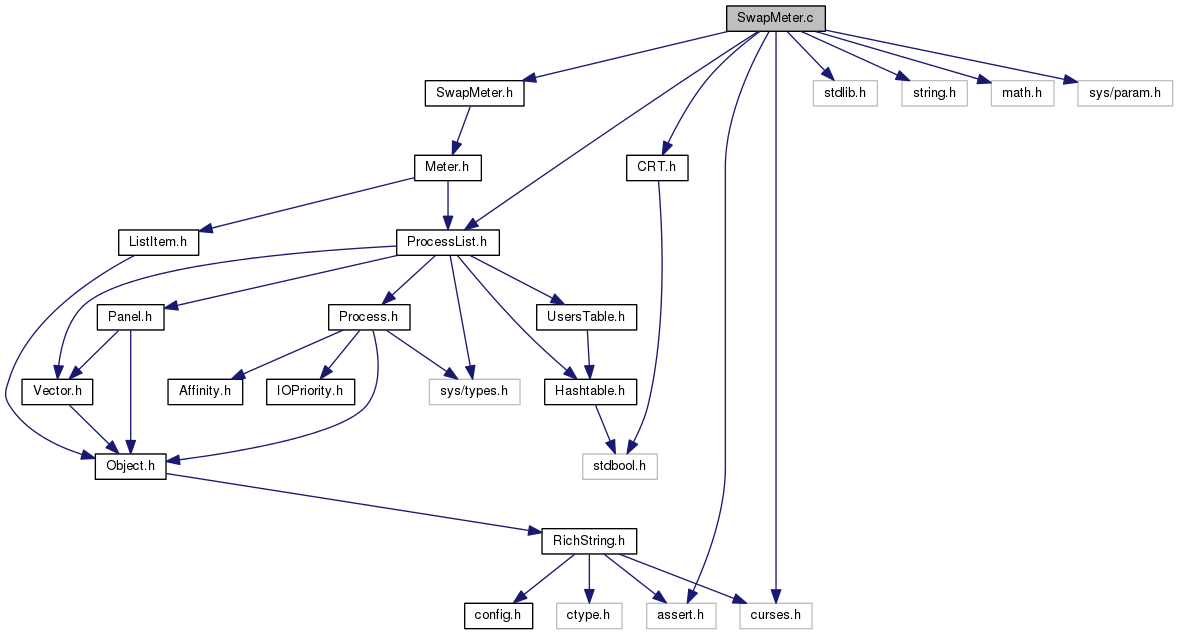
\includegraphics[scale=0.3]{res/swap_meter.png}
\caption{Граф включения для файла SwapMeter.c}
\end{figure}

\end{frame}
%------------------------------------------------
\section{Мониторинг процессов}
%------------------------------------------------

\begin{frame}
\frametitle{Мониторинг процессов}

\begin{figure}
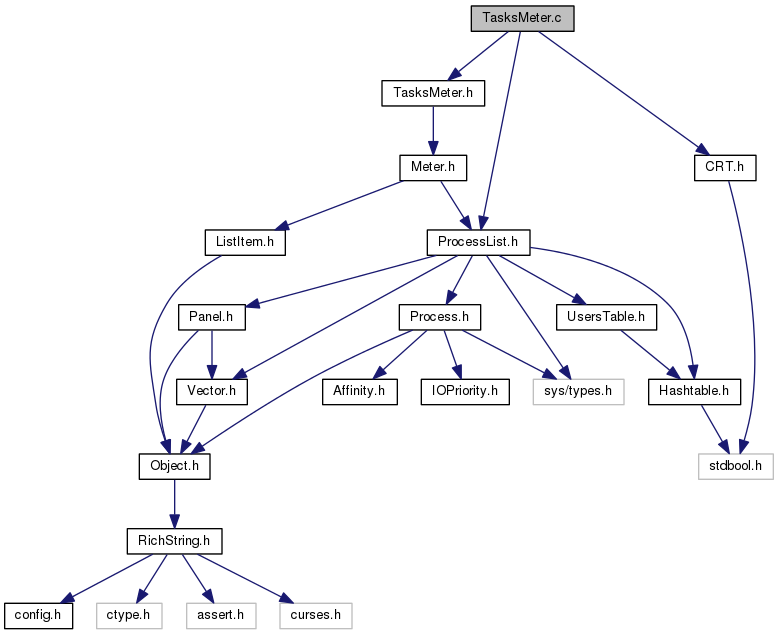
\includegraphics[scale=0.3]{res/tasks_meter.png}
\caption{Граф включения для файла TasksMeter.c}
\end{figure}

\end{frame}
%------------------------------------------------
\section{Измерение времени работы системы}
%------------------------------------------------

\begin{frame}
\frametitle{Измерение времени работы системы}

\begin{figure}
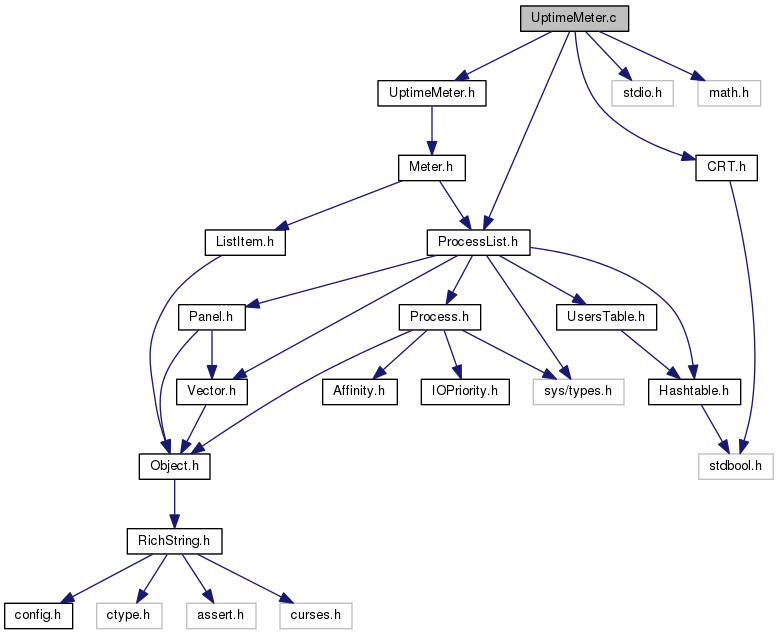
\includegraphics[scale=0.3]{res/uptime_meter.png}
\caption{Граф включения для файла UptimeMeter.c}
\end{figure}

\end{frame}

%------------------------------------------------
\section{Ссылки}
%------------------------------------------------

\begin{frame}
\frametitle{Ссылки}

\begin{itemize}
\item htop - \url{http://hisham.hm/htop/}
\item procps - \url{http://procps.sourceforge.net/}
\end{itemize}

\end{frame}

%------------------------------------------------
\section{Вопросы}
%------------------------------------------------

\begin{frame}
\Huge{\centerline{Вопросы?}}
\end{frame}

%----------------------------------------------------------------------------------------

\end{document} 
